\documentclass{article}
\usepackage{polski}
\usepackage[utf8]{inputenc}
\usepackage{graphics}
\usepackage{graphicx}
\usepackage{wasysym}
\usepackage{mathtools}
\usepackage{amsmath}
\usepackage{breqn}
\usepackage{hyperref}
\usepackage{subfiles}
\usepackage{listings}

\renewcommand\lstlistingname{Kod źródłowy}
\renewcommand\lstlistlistingname{Kod źródłowy}

\usepackage{xcolor}
\definecolor{codegreen}{rgb}{0,0.6,0}
\definecolor{codegray}{rgb}{0.5,0.5,0.5}
\definecolor{codeorange}{rgb}{1,0.49,0}
\definecolor{backcolour}{rgb}{0.95,0.95,0.96}

\lstdefinestyle{mystyle}{
    backgroundcolor=\color{backcolour},
    commentstyle=\color{codegray},
    keywordstyle=\color{codeorange},
    numberstyle=\tiny\color{codegray},
    stringstyle=\color{codegreen},
    basicstyle=\ttfamily\footnotesize,
    breakatwhitespace=false,
    breaklines=false,
    captionpos=t,
    keepspaces=true,
    numbers=left,
    numbersep=5pt,
    showspaces=false,
    showstringspaces=false,
    showtabs=false,
    tabsize=2,
    xleftmargin=10pt,
}
\lstset{style=mystyle}

\title{Goodwin-Griffith-genetic-oscillator-model}
\author{Krzysztof Olech}


\begin{document}

    \maketitle


    Kontrola genów Model zaproponowany przez Griffitha, w którym X to koncentracja pewnego białka proporcjonalna do aktywności opisywanego genu, a Y to koncentracja odpowiedniego mRNA,

    $$\dot{X} = -\alpha X+Y$$

    $$\dot{Y} = \frac{x^2}{1+X^2}-\beta Y$$

    \newpage
    \tableofcontents

    \newpage


    \section{Pkty stale}

    Analize naszego ukladu zaczynamy od analizy pktow stalych. Korzystajac z Wolframa mozemy doknac analizy naszych rownan.

    \subsection{Rowzionzania Trywialne}
    $\alpha$ i $\beta$ = 0

    \begin{figure}[ht]
        \centering
        \begin{minipage}{.5\textwidth}
            \centering
            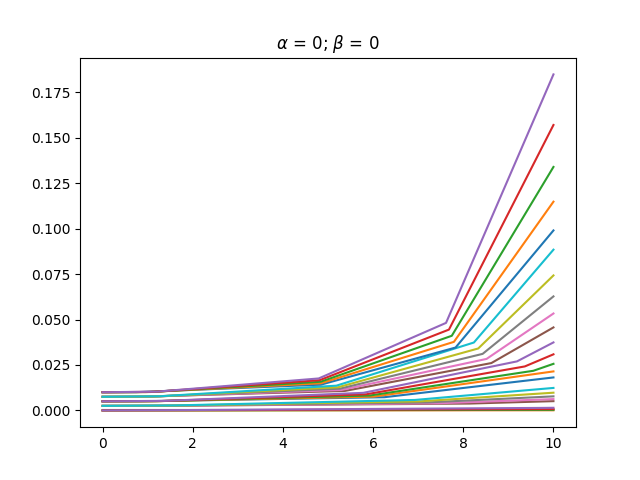
\includegraphics[width=0.8\linewidth]{pktyZerowea=0_b=0_X.png}
            \captionof{}{Wykresy zachowania X}%
            \label{fig:test11}
        \end{minipage}%
        \begin{minipage}{.5\textwidth}
            \centering
            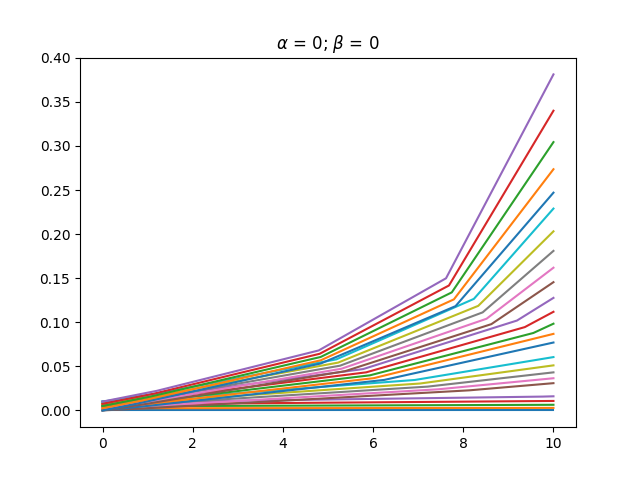
\includegraphics[width=.8\linewidth]{pktyZerowea=0_b=0_Y.png}
            \captionof{}{Wykresy zachowania Y}
            \label{fig:test12}
        \end{minipage}
        \centering
        \begin{minipage}{.5\textwidth}
            \centering
            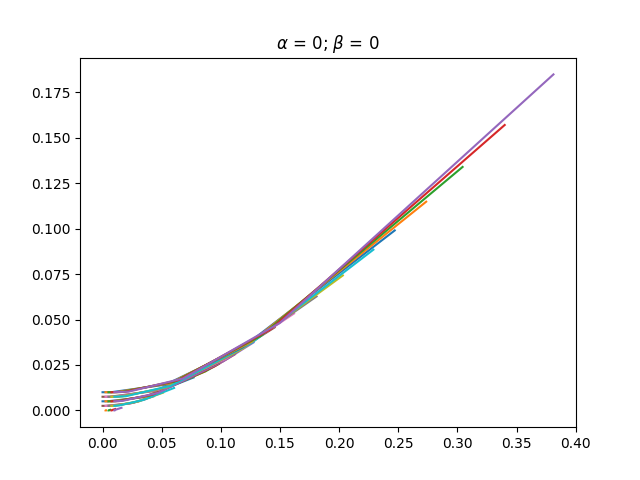
\includegraphics[width=0.8\linewidth]{pktyZerowea=0_b=0_XY.png}
            \captionof{}{Wykres Fazowy}%
            \label{fig:test13}
        \end{minipage}%
    \end{figure}

    Mozemy zaobserwowac ze nasze rozwionzania tylko i wylocznie dla x i y = 0 wiec mozemy wysnuac wniosek ze jest to chwiejny pkt stacionarny postaramy sie potem to udowdonic kozystajac z analizy jakobianu.

    \newpage

    \subsection{Rozwionzania nie trywialne}

    \subsubsection{Przypadek pierwszy}

    \begin{center}
        $X = - \frac{\sqrt{1-4\alpha^2 \beta^2} - 1 }{2\alfa\beta}$ \hspace{0.5cm}
        $Y = - \frac{\sqrt{1-4\alpha^2 \beta^2} - 1 }{2\beta}$
    \end{center}

    \begin{figure}[ht]
        \centering
        \begin{minipage}{.5\textwidth}
            \centering
            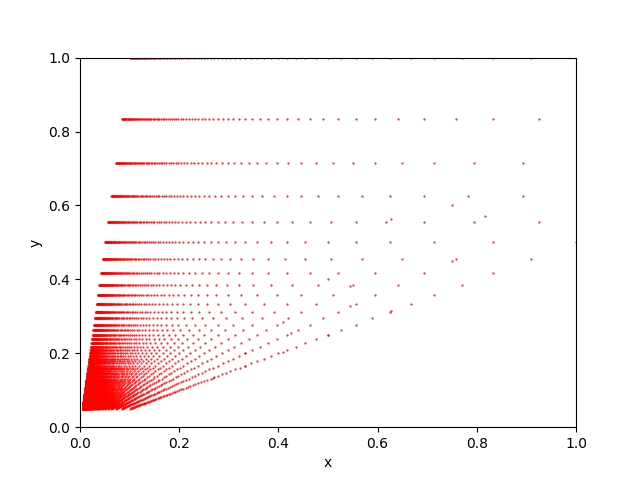
\includegraphics[width=\linewidth]{ujemneNN}
            \captionf{}{a i b in 0.5 do 10}
        \end{minipage}%
        \begin{minipage}{.5\textwidth}
            \centering
            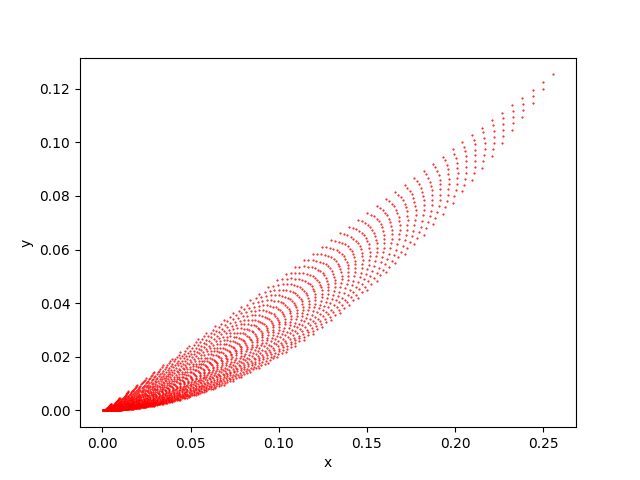
\includegraphics[width=\linewidth]{ujemneNNN}
            \captionf{}{a i b in od 0.01 do 0.5}
        \end{minipage}%
    \end{figure}

    \subsubsection{Przypadek drogi}

    \begin{center}
        $X = \frac{\sqrt{1-4\alpha^2 \beta^2} + 1 }{2\alfa\beta}$\hspace{0.5cm}
        $Y = \frac{\sqrt{1-4\alpha^2 \beta^2} + 1 }{2\beta}$
    \end{center}

    \begin{figure}[ht]
        \centering
        \begin{minipage}{.5\textwidth}
            \centering
            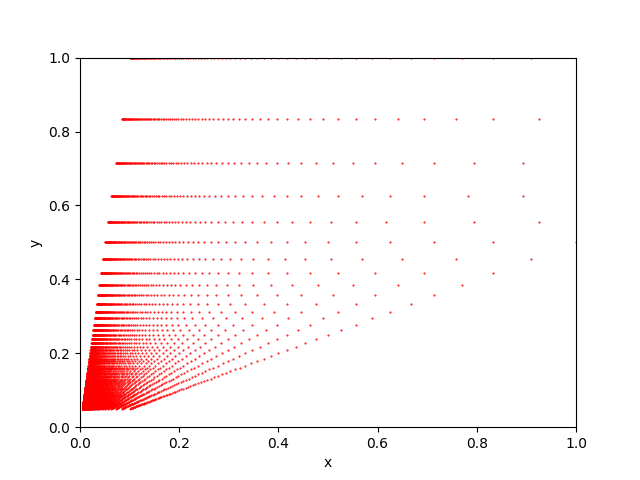
\includegraphics[width=\linewidth]{dodatnieNN}
            \captionf{}{a i b in 0.5 do 10}
        \end{minipage}%
        \begin{minipage}{.5\textwidth}
            \centering
            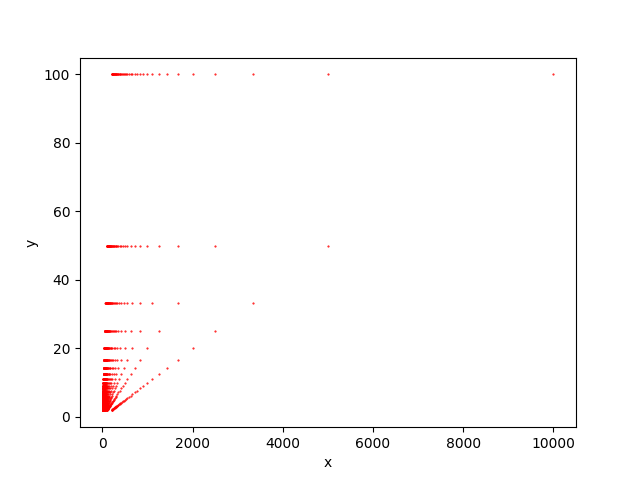
\includegraphics[width=\linewidth]{dodatnieNNN}
            \captionf{}{a i b in 0.01 do 0.5}
        \end{minipage}%
    \end{figure}

    Zastanawiające jest to że dla większych wartości $\alpha$ i $\beta$ pkt stabilne  dla obu równań są dokradnie takie same.

    \newpage
    \subsection{Jakobian}

    \begin{center}
        $$
        \left\{
            \begin{matrix}
                -\alpha & 1 \\
                \frac{2 x}{(x^2+1)^2} & \beta
            \end{matrix}
        \right\}
        $$
    \end{center}

    Potencjalne pkt zerujące równania:\\
    $-\alpha X+Y = 0 \Rightarrow Y = \alpha X$

    $ \frac{x^2}{1+X^2}-\beta Y = 0 \Rightarrow \frac{x^2}{1+X^2} = \beta Y$

    $\frac{x^2}{1+x^2} = \beta  \alpha x$

    rozwiązania:

    trywialne x= 0

    nie trywialne dla $\alpha$ i $\beta \neq 0$

    $x = \frac{1-\sqrt{1 - 4 \alpha^2 \beta^2}}{2 \alpha \beta}$

    $x = \frac{\sqrt{1 - 4 \alpha^2 \beta^2}-1}{2 \alpha \beta}$

    \subsubsection{Rozwiązania dla $x = \frac{1-\sqrt{1 - 4 \alpha^2 \beta^2}}{2 \alpha \beta}$}

    $$
         \lambda_1 =

    (16 \alpha^3 \beta^2
    + 16 \alpha^2 \beta^3
    + 8 \alpha \sqrt{1 - 4 \alpha^2 \beta^2}
    + 8 \beta \sqrt{1 - 4 \alpha^2 \beta^2}

    \vspace{0.5cm}
    -\sqrt{
        (-16 \alpha^3 \beta^2
        - 16 \alpha^2 \beta^3
        - 8 \alpha \sqrt{1 - 4 \alpha^2 \beta^2}
        - 8 \beta \sqrt{1 - 4 \alpha^2 \beta^2}
        + 8 \alpha + 8 \beta)^2

        \vspace{0.5cm}
        \overline{- 4 (1024 \alpha^5 \beta^5
            - 768 \alpha^3 \beta^3
            - 128 \alpha \beta \sqrt{1 - 4 \alpha^2 \beta^2)}
            - 256 \alpha^5 \beta^5 \sqrt{1 - 4 \alpha^2 \beta^2}}

        \vspace{0.5cm}
        \overline{
            + 512 \alpha^3 \beta^3 \sqrt{1 - 4 \alpha^2 \beta^2}
            + 128 \alpha \beta)
            )}
        - 8 \alpha
        - 8 \beta
        }

    \vspace{0.5cm}
    /(2 (2 - 2 \sqrt{1 - 4 \alpha^2 \beta^2})^2)
    $$

    $$
    \lambda_2 =

    (16 \alpha^3 \beta^2
    + 16 \alpha^2 \beta^3
    + 8 \alpha \sqrt{1 - 4 \alpha^2 \beta^2}
    + 8 \beta \sqrt{1 - 4 \alpha^2 \beta^2}

    \vspace{0.5cm}
    + \sqrt{
            (-16 \alpha^3 \beta^2
            - 16 \alpha^2 \beta^3
            - 8 \alpha \sqrt{1 - 4 \alpha^2 \beta^2}
            - 8 \beta \sqrt{1 - 4 \alpha^2 \beta^2}
            + 8 \alpha + 8 \beta)^2

        \vspace{0.5cm}
        \overline{
        - 4 (
            1024 \alpha^5 \beta^5
            - 768 \alpha^3 \beta^3
            - 128 \alpha \beta \sqrt{1 - 4 \alpha^2 \beta^2}
            - 256 \alpha^5 \beta^5 \sqrt{1 - 4 \alpha^2 \beta^2}
            + 512 \alpha^3 \beta^3 \sqrt{1 - 4 \alpha^2 \beta^2}
            + 128 \alpha \beta)
    }}

    \vspace{0.5cm}
    - 8 \alpha
    - 8 \beta)

    \vspace{0.5cm}
    /(2 (2 - 2 \sqrt{1 - 4 \alpha^2 \beta^2})^2)
    $$


    \subsubsection{Rozwiązania dla $x = \frac{\sqrt{1 - 4 \alpha^2 \beta^2}-1}{2 \alpha \beta}$}

    $$
    \lambda_1 =

    (16 \alpha^3 \beta^2
    + 16 \alpha^2 \beta^3
    + 8 \alpha \sqrt{1 - 4 \alpha^2 \beta^2}
    + 8 \beta \sqrt{1 - 4 \alpha^2 \beta^2}

    \vspace{0.5cm}
    - \sqrt{
        (
            -16 \alpha^3 \beta^2
            - 16 \alpha^2 \beta^3
            - 8 \alpha \sqrt{1 - 4 \alpha^2 \beta^2}
            - 8 \beta \sqrt{1 - 4 \alpha^2 \beta^2}
            + 8 \alpha
            + 8 \beta
        )^2

        \vspace{0.5cm}
        \overline{
        - 4 (
            -512 \alpha^5 \beta^5
            - 256 \alpha^3 \beta^3
            - 128 \alpha \beta \sqrt{1 - 4 \alpha^2 \beta^2}
            + 256 \alpha^5 \beta^5 \sqrt{1 - 4 \alpha^2 \beta^2}
            + 128 \alpha \beta
        )
    }}

        \vspace{0.5cm}
        - 8 \alpha
        - 8 \beta
    )
    /(2 (2 - 2 \sqrt{1 - 4 \alpha^2 \beta^2})^2)
    $$

    $$
    \lambda_2 =

    (16 \alpha^3 \beta^2
    + 16 \alpha^2 \beta^3
    + 8 \alpha \sqrt{1 - 4 \alpha^2 \beta^2}
    + 8 \beta \sqrt{1 - 4 \alpha^2 \beta^2}

    \vspace{0.5cm}
    + \sqrt{
        (
            -16 \alpha^3 \beta^2
            - 16 \alpha^2 \beta^3
            - 8 \alpha \sqrt{1 - 4 \alpha^2 \beta^2}
            - 8 \beta \sqrt{1 - 4 \alpha^2 \beta^2}
            + 8 \alpha
            + 8 \beta
        )^2

    \vspace{0.5cm}
    \overline{
    - 4 (
        -512 \alpha^5 \beta^5
        - 256 \alpha^3 \beta^3
        - 128 \alpha \beta \sqrt{1 - 4 \alpha^2 \beta^2}
        + 256 \alpha^5 \beta^5 \sqrt{1 - 4 \alpha^2 \beta^2}
        + 128 \alpha \beta)
    }}

    \vspace{0.5cm}
    - 8 \alpha
    - 8 \beta
    )
    /(2 (2 - 2 \sqrt{1 - 4 \alpha^2 \beta^2})^2)
    $$


    Niestety rozwiązanie Tych równań jest bardzo zmożone i cienkie dlatego nie wykonamy analizy stabilności Kotow stałych z ich pomocą lecz wykonamy to numerycznie.

    Próba znalezienia numerycznego rozwiązania nie udała się ze względu na niska ilość algorytmów umożliwiających analizę równań uwikłanych. Dostępne są za peywalem na matematice.

    załącznik 1.


\newpage

    \section{analiza}
        Pierwsze wykresy zostały stworzone dla szerokiego zakresu pkt x i y dla kilku stałych a i b
        Załącznik 2.

    \subsection{$\alpha=0.5$ $\beta=0.5$}
    x i y początkowe z zakresu od 0.1 do 1 (wsystkei kombinacje co około 0.01)
            \begin{figure}[ht]
        \centering
        \begin{minipage}{.5\textwidth}
            \centering
            \includegraphics[width=0.8\linewidth]{DuzyZakres=0.5_b=0.5_X.png}
            \captionof{}{Wykresy zachowania X}%
            \label{fig:test11}
        \end{minipage}%
        \begin{minipage}{.5\textwidth}
            \centering
            \includegraphics[width=.8\linewidth]{DuzyZakres=0.5_b=0.5_Y.png}
            \captionof{}{Wykresy zachowania Y}
            \label{fig:test12}
        \end{minipage}
        \centering
        \begin{minipage}{.5\textwidth}
            \centering
            \includegraphics[width=0.8\linewidth]{DuzyZakres=0.5_b=0.5_XY.png}
            \captionof{}{Wykres Fazowy}%
            \label{fig:test13}
        \end{minipage}%
    \end{figure}

    \newpage
    \subsection{$\alpha=0.55$ $\beta=0.55$}
    x i y początkowe z zakresu od 0.7 do 0.71
            \begin{figure}[ht]
        \centering
        \begin{minipage}{.5\textwidth}
            \centering
            \includegraphics[width=0.8\linewidth]{DuzyZakres=0.55_b=0.55_X.png}
            \captionof{}{Wykresy zachowania X}%
            \label{fig:test11}
        \end{minipage}%
        \begin{minipage}{.5\textwidth}
            \centering
            \includegraphics[width=.8\linewidth]{DuzyZakres=0.55_b=0.55_Y.png}
            \captionof{}{Wykresy zachowania Y}
            \label{fig:test12}
        \end{minipage}
        \centering
        \begin{minipage}{.5\textwidth}
            \centering
            \includegraphics[width=0.8\linewidth]{DuzyZakres=0.55_b=0.55_XY.png}
            \captionof{}{Wykres Fazowy}%
            \label{fig:test13}
        \end{minipage}%
    \end{figure}

    \newpage
    \subsection{$\alpha=0.45$ $\beta=0.45$}
    x i y początkowe z zakresu od 0.7 do 0.71
            \begin{figure}[ht]
        \centering
        \begin{minipage}{.5\textwidth}
            \centering
            \includegraphics[width=0.8\linewidth]{DuzyZakres=0.45_b=0.45_X.png}
            \captionof{}{Wykresy zachowania X}%
            \label{fig:test11}
        \end{minipage}%
        \begin{minipage}{.5\textwidth}
            \centering
            \includegraphics[width=.8\linewidth]{DuzyZakres=0.45_b=0.45_Y.png}
            \captionof{}{Wykresy zachowania Y}
            \label{fig:test12}
        \end{minipage}
        \centering
        \begin{minipage}{.5\textwidth}
            \centering
            \includegraphics[width=0.8\linewidth]{DuzyZakres=0.45_b=0.45_XY.png}
            \captionof{}{Wykres Fazowy}%
            \label{fig:test13}
        \end{minipage}%
    \end{figure}

    \newpage
    \subsection{$\alpha=0.6$ $\beta=0.6$}
    x i y początkowe z zakresu od 0.5 do 1
            \begin{figure}[ht]
        \centering
        \begin{minipage}{.5\textwidth}
            \centering
            \includegraphics[width=0.8\linewidth]{DuzyZakres=0.6_b=0.6_X.png}
            \captionof{}{Wykresy zachowania X}%
            \label{fig:test11}
        \end{minipage}%
        \begin{minipage}{.5\textwidth}
            \centering
            \includegraphics[width=.8\linewidth]{DuzyZakres=0.6_b=0.6_Y.png}
            \captionof{}{Wykresy zachowania Y}
            \label{fig:test12}
        \end{minipage}
        \centering
        \begin{minipage}{.5\textwidth}
            \centering
            \includegraphics[width=0.8\linewidth]{DuzyZakres=0.6_b=0.6_XY.png}
            \captionof{}{Wykres Fazowy}%
            \label{fig:test13}
        \end{minipage}%
    \end{figure}

    \newpage
    \subsection{$\alpha=1$ $\beta=1$}
    x i y początkowe z zakresu od 0.5 do 1
            \begin{figure}[ht]
        \centering
        \begin{minipage}{.5\textwidth}
            \centering
            \includegraphics[width=0.8\linewidth]{DuzyZakres=1_b=1_X.png}
            \captionof{}{Wykresy zachowania X}%
            \label{fig:test11}
        \end{minipage}%
        \begin{minipage}{.5\textwidth}
            \centering
            \includegraphics[width=.8\linewidth]{DuzyZakres=1_b=1_Y.png}
            \captionof{}{Wykresy zachowania Y}
            \label{fig:test12}
        \end{minipage}
        \centering
        \begin{minipage}{.5\textwidth}
            \centering
            \includegraphics[width=0.8\linewidth]{DuzyZakres=1_b=1_XY.png}
            \captionof{}{Wykres Fazowy}%
            \label{fig:test13}
        \end{minipage}%
    \end{figure}


        \newpage
    \subsection{$\alpha=5$ $\beta=5$}
    x i y początkowe z zakresu od 0 do 10
            \begin{figure}[ht]
        \centering
        \begin{minipage}{.5\textwidth}
            \centering
            \includegraphics[width=0.8\linewidth]{DuzyZakres=5_b=5_X.png}
            \captionof{}{Wykresy zachowania X}%
            \label{fig:test11}
        \end{minipage}%
        \begin{minipage}{.5\textwidth}
            \centering
            \includegraphics[width=.8\linewidth]{DuzyZakres=5_b=5_Y.png}
            \captionof{}{Wykresy zachowania Y}
            \label{fig:test12}
        \end{minipage}
        \centering
        \begin{minipage}{.5\textwidth}
            \centering
            \includegraphics[width=0.8\linewidth]{DuzyZakres=5_b=5_XY.png}
            \captionof{}{Wykres Fazowy}%
            \label{fig:test13}
        \end{minipage}%
    \end{figure}

    \newpage
    \subsection{$\alpha=0.5$ $\beta=0.5$}
    x i y początkowe z zakresu od 0 do 100
            \begin{figure}[ht]
        \centering
        \begin{minipage}{.5\textwidth}
            \centering
            \includegraphics[width=0.8\linewidth]{DuzyZakres_2=0.5_b=0.5_X.png}
            \captionof{}{Wykresy zachowania X}%
            \label{fig:test11}
        \end{minipage}%
        \begin{minipage}{.5\textwidth}
            \centering
            \includegraphics[width=.8\linewidth]{DuzyZakres_2=0.5_b=0.5_Y.png}
            \captionof{}{Wykresy zachowania Y}
            \label{fig:test12}
        \end{minipage}
        \centering
        \begin{minipage}{.5\textwidth}
            \centering
            \includegraphics[width=0.8\linewidth]{DuzyZakres_2=0.5_b=0.5_XY.png}
            \captionof{}{Wykres Fazowy}%
            \label{fig:test13}
        \end{minipage}%
    \end{figure}

    \newpage
    \subsection{$\alpha=0.5$ $\beta=0.5$}
    x i y początkowe z zakresu od-100 do 0 - nie rzeczywisty zakres stężenie białka ujemne
            \begin{figure}[ht]
        \centering
        \begin{minipage}{.5\textwidth}
            \centering
            \includegraphics[width=0.8\linewidth]{DuzyZakres_3=0.5_b=0.5_X.png}
            \captionof{}{Wykresy zachowania X}%
            \label{fig:test11}
        \end{minipage}%
        \begin{minipage}{.5\textwidth}
            \centering
            \includegraphics[width=.8\linewidth]{DuzyZakres_3=0.5_b=0.5_Y.png}
            \captionof{}{Wykresy zachowania Y}
            \label{fig:test12}
        \end{minipage}
        \centering
        \begin{minipage}{.5\textwidth}
            \centering
            \includegraphics[width=0.8\linewidth]{DuzyZakres_3=0.5_b=0.5_XY.png}
            \captionof{}{Wykres Fazowy}%
            \label{fig:test13}
        \end{minipage}%
    \end{figure}

    \subsection{Wnioski}
    Analizując nie rzeczywiste wyniki możemy ustalić ze na pewno po stronie ujemnej pkt x y = 0 jest atraktorem dla nie za duzych dodatnich zmiennych x i y jest atraktorem również po dodatniej stronie.


    \newpage
    \section{Bifurkacje}

    Poszukiwanie pktu podejrzanego o Bifurkacje.
    Po napisaniu Kodu umozliwiajacego liczenie mi Bifurkacje załącznik 3 zaczełem szukac czy istnieje pkt w któym wystompi Bifurkacja.

    \subsection{$\alpha$ w zakresie od 0 do 500}
    \begin{figure}[ht]
        \centering
        \begin{minipage}{.5\textwidth}
            \centering
            \includegraphics[width=0.8\linewidth]{a=10, b=10, x=0.5, y=0.5, z=a, i= 999, j= x.png}
            \captionof{}{Wykresy zachowania X}%
            \label{fig:test11}
        \end{minipage}%
        \begin{minipage}{.5\textwidth}
            \centering
            \includegraphics[width=.8\linewidth]{a=10, b=10, x=0.5, y=0.5, z=a, i= 999, j= y.png}
            \captionof{}{Wykresy zachowania Y}
            \label{fig:test12}
        \end{minipage}
    \end{figure}

        \subsection{$\beta$ w zakresie od 0 do 500}
    \begin{figure}[ht]
        \centering
        \begin{minipage}{.5\textwidth}
            \centering
            \includegraphics[width=0.8\linewidth]{a=10, b=1, x=0.5, y=0.5, z=a, i= 999, j= x.png}
            \captionof{}{Wykresy zachowania X}%
            \label{fig:test11}
        \end{minipage}%
        \begin{minipage}{.5\textwidth}
            \centering
            \includegraphics[width=.8\linewidth]{a=10, b=1, x=0.5, y=0.5, z=a, i= 999, j= y.png}
            \captionof{}{Wykresy zachowania Y}
            \label{fig:test12}
        \end{minipage}
    \end{figure}

    \newpage
    \subsection{$\alpha$ w zakresie od 0 do 1, 10k pkt}
    \begin{figure}[ht]
        \centering
        \begin{minipage}{.5\textwidth}
            \centering
            \includegraphics[width=0.8\linewidth]{a=0.5, b=0.5, x=0.5, y=0.5, z=a, i= 9999, j= x.png}
            \captionof{}{Wykresy zachowania X}%
            \label{fig:test11}
        \end{minipage}%
        \begin{minipage}{.5\textwidth}
            \centering
            \includegraphics[width=.8\linewidth]{a=0.5, b=0.5, x=0.5, y=0.5, z=a, i= 9999, j= y.png}
            \captionof{}{Wykresy zachowania Y}
            \label{fig:test12}
        \end{minipage}
    \end{figure}

        \subsection{$\beta$ w zakresie od 0 do 1, 10k pkt}
    \begin{figure}[ht]
        \centering
        \begin{minipage}{.5\textwidth}
            \centering
            \includegraphics[width=0.8\linewidth]{a=0.5, b=0.5, x=0.5, y=0.5, z=b, i= 9999, j= x.png}
            \captionof{}{Wykresy zachowania X}%
            \label{fig:test11}
        \end{minipage}%
        \begin{minipage}{.5\textwidth}
            \centering
            \includegraphics[width=.8\linewidth]{a=0.5, b=0.5, x=0.5, y=0.5, z=b, i= 9999, j= y.png}
            \captionof{}{Wykresy zachowania Y}
            \label{fig:test12}
        \end{minipage}
    \end{figure}

    \newpage

    \subsection{Wnioski}
        Możemy zaobserwować brak bifurkacji dla sprawdzanych parametrów oraz możemy zaobserwować ze istnieją nie ciągłości funkcji dla kilku pktów w szczególności w okolicach $\beta$ = 0.3 oraz $\alpha$ = 0.18 które mogły by sugerować możliwość zaistnienia bifurkacji w okolicach tamtego pkt niestety nie udało mi się ich wyznaczyć a z uwagi na brak analitycznego określenia pktów stałych nie byłem w stanie dokładniej ich określić zęby stwierdzić czy są możliwe.

\section{Wnioski}
    Niestety z uwagi na niska znajomość procesów biologicznych z mojej strony nie dokona dobrze zrozumiałem model Biologiczny który był symulowany. Wiem ze zmienne x i y określają stężenia określonych protein. Za to parametry $\alpha$ i $\beta$ określają prędkości wymiany określonych protein. W głównej publikacji rozważano dużo bardziej złożone równania niż te które ja rozważałem. Możliwe ze brak oscylacji lub jej bardzo szybkie tłumienie sprowadza się do tego lub za niskiej dokładności pakietu użytego do całkowania.

\newpage
    \section{Załączniki}

        \url{https://github.com/KrOlech/Goodwin-Griffith-genetic-oscillator-model}

        \subsection{Załącznik 0}
        \lstinputlisting[language=Python, caption={Uniwersalne Funkcje.},label={lst:pmv_example}, mathescape=true]{UniversalFun.py}

        \newpage
        \subsection{Załącznik 1}
        \lstinputlisting[language=Python, caption={Pkty Zerowe Funkcji.},label={lst:pmv_example}, mathescape=true]{PktyStabilne.py}

        \newpage
        \subsection{Załącznik 1.5}
        \lstinputlisting[language=Python, caption={Pkty Zerowe Funkcji Próba okreslenia stabilnosci.},label={lst:pmv_example}, mathescape=true]{pktyZerowe.py}


        \newpage
        \subsection{Załącznik 2}
        \lstinputlisting[language=Python, caption={Pierwsze sprawdzenie dla stałego $\alpha$ i $\beta$.},label={lst:pmv_example}, mathescape=true]{szerokiZakres.py}

        \newpage
        \subsection{Załącznik 3}
        \lstinputlisting[language=Python, caption={Bifurkacje.},label={lst:pmv_example}, mathescape=true]{MainFunctions.py}



ł
        \newpage
        \subsection{Uruchomienie}
        Załącznik zerowy jest konieczny w ramach odpalenia załącznika 2 i 3.

        Żeby wykonac kazdy z plików nalezy zainstalwoac Pythona (w wykonaniu był uzywany python 3.10 ale program powinien działac poprawnie równiez na wersji 3.8 i wyzej)
        Oraz pakiety do Pythona:
        -numpy
        -Scipy
        -Matplotlib

        Programy pracują wielowątkowo, Dokładniej wieloprocesowo gdyż niestety jak na razie Python nie wspiera w pełni wielowontkowosci planują to zmienić w ramach wersji 3.12 lub 3.13. Ilość procesów została ustalona na 10 jako ze tyle pozwalał mój procesor bez problemów z używaniem komputera w trakcie działania programu. W celu zmienienia tego należy edytować odpowiedni parametr w programie. Nie powiano być problemu z włączaniem programu z nisza ilością rdzeni lecz mogą pojawić się komunikaty o błędach i wyniki mogą być nie kompletne.

        Każdy z pod programów wykona i zapisze do pliku wykresy o nazwach w określonej konwencji.
\end{document}
